%%%%%%%%%%%%%%%%%%%%%%%%%%%%%%%%%%%%%%%%%%%%%%%%%%%%%%%%%%%%%%%%%%%%%%%%
%    INSTITUTE OF PHYSICS PUBLISHING                                   %
%                                                                      %
%   `Preparing an article for publication in an Institute of Physics   %
%    Publishing journal using LaTeX'                                   %
%                                                                      %
%    LaTeX source code `ioplau2e.tex' used to generate `author         %
%    guidelines', the documentation explaining and demonstrating use   %
%    of the Institute of Physics Publishing LaTeX preprint files       %
%    `iopart.cls, iopart12.clo and iopart10.clo'.                      %
%                                                                      %
%    `ioplau2e.tex' itself uses LaTeX with `iopart.cls'                %
%                                                                      %
%%%%%%%%%%%%%%%%%%%%%%%%%%%%%%%%%%%%%%%%%%%%%%%%%%%%%%%%%%%%%%%%%%%%%%%%

% Document class definition
\documentclass[12pt]{iopart}

% Addition of neater URL's and hyperrefs
\usepackage{url} 

% better encoding of text
\usepackage[utf8]{inputenc}
\usepackage[T1]{fontenc}

% Addition of linenumbers 
\usepackage{lineno} 
\linenumbers

% for nicer non-forced page breaks
\usepackage{afterpage}

% for nicer lists
\usepackage{enumitem}

% A short-hand for superscripting
\newcommand{\ts}[1]{\textsuperscript{#1}}

% short-hand for the index name
\newcommand{\credi}[0]{{\sc credi}}
\newcommand{\sdi}[0]{{\sc solar credi}}
\newcommand{\wdi}[0]{{\sc wind credi}}

% nicer figures
\usepackage{graphicx}

% Determine bibliography 
\usepackage[style=authoryear,backend=biber]{biblatex}
\addbibresource{sample.bib}




% Start of the document
\begin{document}

% Title
\title[The Climatological Renewable Energy Deviation Index]{The Climatological Renewable Energy Deviation Index}

% Author list
\author{Laurens P. Stoop$^{1,2,3,A}$, Karin van der Wiel$^{4,B}$, William Zappa$^{3,N}$, Arno Haverkamp$^{3,O}$, Ad J. Feelders$^{1,Y}$ and Machteld van den Broek$^{4,Z}$}

% Adresses
\address{$^1$ Information and Computing Science, Utrecht University, the Netherlands}
\address{$^2$ Copernicus Institute of Sustainable Development, Utrecht University, the Netherlands}
\address{$^3$ TenneT TSO B.V., Arnhem, the Netherlands}
\address{$^4$ Royal Netherlands Meteorological Institute (KNMI), the Netherlands}
\address{$^5$ Integrated Research on Energy, Environment and Society, Energy and Sustainability Research Institute Groningen (ESRIG), University of Groningen, the Netherlands}

% ORCiD listings
\orcid{$^A$ 0000-0003-2756-5653}
\orcid{$^B$ 0000-0001-9365-5759}
\orcid{$^N$ 0000-0001-6810-7224}
\orcid{$^O$ 0000-0001-6947-7892}
\orcid{$^Y$ 0000-0003-4525-1949}
\orcid{$^Z$ 0000-0003-1028-1742}

% Contact info
\ead{l.p.stoop@uu.nl}
\vspace{10pt}
\begin{indented}
\item[]July 2023
\end{indented}

%%%%%%%%%%%%%%%%%%%%%%%%%%%%%%%%%%%%%%%%%%%%%%%%%%
%%%%		~~~~ Abstract ~~~~
%%%%%%%%%%%%%%%%%%%%%%%%%%%%%%%%%%%%%%%%%%%%%%%%%%

\begin{abstract}
% Context & inspiration
Here we propose an index to quantify and analyse the impact of climatological variability on the energy system at different timescales.
% Definition
We define the Climatological Renewable Energy Deviation Index (\credi) as the cumulative anomaly of a renewable resource with respect to its climate over a specific time period of interest.
% Possible applications  & considerations
We analyse the index at decadal, annual and (sub-)seasonal timescales using the forthcoming Pan-European Climate Database and consider the starting point and window of analysis for its use at those timescales.
% use of CREBI later Users, Use and Application
The \credi{} is meant as an analytical tool for researchers and stakeholders to help them quantify, understand, and explain, the impact of the variability of weather on the energy system across timescales. 
Improved understanding translates to better assessments of how renewable resources, and the associated risks for energy security, may fare in current and future climatological settings.
The practical use of the index is in resource planning. 
For example transmission system operators may be able to adjust short-term planning to reduce adequacy issues before they occur or combine the index with storyline event selection for improved assessments of climate change related risks.
\end{abstract}


% Additional keywords
\vspace{2pc}
\noindent{\it Keywords}: Variability, Resource Adequacy, Renewable Energy Drought, Dunkelflaute, Wind Drought

% Submitted to journal title message
\submitto{\ERL}
% ERL would mean 4000 words max

% Uncomment if a separate title page is required
\maketitle



%%%%%%%%%%%%%%%%%%%%%%%%%%%%%%%%%%%%%%%%%%%%%%%%%%
%%%%		~~~~ Introduction ~~~~
%%%%%%%%%%%%%%%%%%%%%%%%%%%%%%%%%%%%%%%%%%%%%%%%%%

\section{Introduction}
% the Energy transition is here, it brings more variability / dynamics
The energy system is changing. 
This is due to the increased deployment of renewable energy generators, like wind turbines and solar panels; changes in electricity demand, from increased use of heat pumps and electric vehicles; and climatic changes influencing the weather dependent parts of the system. 
It is crucial to understand the full dynamics of the (future) energy system, both for policy making and energy security reasons~\autocite{craig2022disconnect}.

% Energy-meteo Variability  description
Knowing the impact of and link between the energy system and weather-related variability on daily to inter-annual and decadal timescales is vital for robust design and planning of future energy systems~\autocite{Bloomfield2021nextgen,craig2022disconnect,McKenna2022}. 
Meteorological variability leads to temporal variability. 
Not only in renewable energy production, but also in energy demand, changing the way energy systems have to be operated and controlled~\autocite{craig2022disconnect}.

% We need ESM's but to complex
Energy system models are vital to capture the impact of this variability~\parencite{gernaat2021climate}. 
However, their complexity results in high computational burdens that grows exponentially with the simulation period~\parencite{wuijts2022modelchar,Price2022,craig2022disconnect,wuijts2023linking,Grochowicz2023}. 
Incorporating large climate datasets that capture meteorological variability in \emph{operational hourly} energy system models is thus, as of yet, unfeasible~\parencite{Harang2020,craig2022disconnect,wuijts2023linking}. 
Even so, understanding meteorological variability, i.e. potential challenging events and their drivers, can aid  system operators in their task to ensure both short- and long-term energy security~\parencite{craig2022disconnect,wuijts2023linking,Hu2023}. 
Therefore, alternative approaches are needed to assess energy-meteorological variability~\parencite{craig2022disconnect,Dubus2022PECD}. 
While a number of methods exists to model and/or select challenging high impact events~\parencite[e.g.][]{vanderwiel2019extreme,Ohlendorf2020,OteroFelipe2021,stoop2021detection,vanderMost2022,Boston2022,Hu2023}, we aim to define a metric to quantify energy-meteorological variability across timescales.

% Inter-annual and decadal variability captured in hydrology in 'neerslagtekort'
In our quest to develop this metric, we were inspired by the hydrological sciences. 
For drought monitoring, a number of indices have proven useful for both scientific assessment and operational use. 
These drought indices, such as the Climatological Water Balance~\parencite[CWB;][]{gleick1985regional,Gleick1986}, the Standardised Precipitation Index \parencite[SPI;][]{mckee1993}, and the Standardised Precipitation-Evapotranspiration Index \parencite[SPEI;][]{VicenteSerrano2010}), are based on precipitation deficits (anomaly of precipitation, or anomaly of the difference between potential evapotranspiration and precipitation) and are used to assess the temporal development of dry or wet periods. 
Furthermore, they have been used to assess the influence of inter-annual to multi-decadal variability, and of climate change on the temporal variability of hydrological drought~\parencite[e.g.][]{Quiring2009,Stagge2015,Cammalleri2021,vanderWiel2022}. 
Some aspects of these indices and their use in assessing hydrological variability can be transferred to the energy-meteorological domain.

% inspired by CWB we define CREDI
We define the Climatological Renewable Energy Deviation Index (\credi) as the cumulative anomaly of a renewable resource with respect to its climate over a specific time period of interest (Figure~\ref{fig:overview}). 
Given this definition, this study addresses the following considerations: (a) how do you define the climatic behaviour of a highly variable renewable resource, like wind or solar? and (b) how do you analyse this index at different timescales; like (sub-)seasonal, annual, or multi-decadal?

\begin{figure}[b]
        \centering
        \includegraphics[width=\textwidth]{Figures/Schematic_CREDI.pdf}
        % \includegraphics[width=\textwidth]{MainMatter/CP2/Figures/Schematic_CREDI.pdf}
        \caption{
                Illustration of climatological renewable energy deviation index. 
                Given the climate of a renewable resource (black line in panel~a), the instantaneous anomaly can be calculated (orange/teal bars in panel~a). 
                Positive anomalies (orange) increase and negative anomalies (teal) decrease the index, which starts at zero at the start of period of analysis (panel~b). 
                Illustration shows solar potential anomalies for 2021 with respect to a 1991-2020 climate, and the \sdi{} with a starting point at 1~March. 
                Two meteorological forecast ensemble members converted to \credi{} are shown to indicate a use-case for grid-operators. }
        \label{fig:overview}
\end{figure}

% structure
The paper is structured as follows. 
In Section~\ref{secCP2:clima}, we define the renewable resource climate and the index. 
In Section~\ref{secCP2:analysis}, we analyse the index at different timescales and discuss the best starting point. 
In the Section~\ref{secCP2:discussion} we discuss our definition of the index. 
Finally, in Section~\ref{secCP2:conclusion}, a synthesis of our findings is presented and potential use cases in research and/or operational application are outlined. 
Supporting Information (SI) with additional figures and observational analysis is available online.





%%%%%%%%%%%%%%%%%%%%%%%%%%%%%%%%%%%%%%%%%%%%%%%%%%
%%%%		~~~~ Method ~~~~
%%%%%%%%%%%%%%%%%%%%%%%%%%%%%%%%%%%%%%%%%%%%%%%%%%

\section{Definition of the climatic characterisation and index}\label{secCP2:clima}

% What is climate?
Within the atmospheric sciences the climate of a region is defined as the statistical-mean weather conditions prevailing in that region~\parencite{Arguez2011}. 
% Knowing this climate is useful to benchmark observed conditions, or as an indicator of weather to come. 
The \textcite[WMO;][]{wmo2017normals} has a standardised method for calculation of the \emph{climatological normals}, which comes down to calculating monthly or daily mean values over a 30-year period. 
The climate, or mean expected behaviour, of renewable resources could be defined similarly. 
However, monthly or daily climatological values are not suitable due to the highly variable nature of renewable resources like wind and solar energy, and the need to balance the power grid at shorter timescales.

% Relevant timescales for Energy-meteo variability
We can distinguish four relevant timescales that cover the main modes of energy-meteorological variability. 
Namely:
\begin{enumerate}
        \item annual to decadal timescales: variability caused by interactions in the coupled ocean-atmosphere-system, e.g. modes of variability like the El-Ni\~no-Southern Oscillation \parencite[ENSO;][]{ipcc6_wg1_variability} or the North Atlantic Oscillation \parencite[NAO;][]{Wanner2001},
        \item seasonal timescale: variability caused by the revolution of the Earth around the Sun and the directly related variation of the solar declination angle,
        \item sub-seasonal timescale: variability caused by the cumulative interplay at various timescales, associated with the passing of weather systems and the changes in their persistence and occurrence,
        \item daily timescale: variability caused by the revolution of the Earth around its axis, and the directly related times of sunrise, sunset, and the solar elevation angle.
\end{enumerate}
When studying the generation potential of wind or solar, all these timescales of variability should be considered.


%%%%%%%%%%%%%%%%%%%%%%%%%%%%%%%%%%%%%%%%%%%%%%%%%%
%%%%		~~~~ Definition: Variability

\subsection{Observed variability of wind and solar energy potential}\label{secCP2:variability}
Examples of typical behaviour of wind and solar energy are shown in Figure~\ref{fig:climatological_behaviour}. 
For wind, at seasonal timescales, we observe lower mean generation potential in the summer period (Figure~\ref{fig:climatological_behaviour}a, \ref{fig:climate}a), when weather conditions are more stable. 
The higher and more variable generation potential in the autumn and winter period is associated with the quicker succession of storms in Europe (Figure~\ref{fig:climatological_behaviour}a,b).

% paragraph brake (it was a bit long)
For solar the difference between summer and winter is more pronounced, which is predominantly due to seasonal changes in the angle of declination of the sun (Figure~\ref{fig:climatological_behaviour}d and \ref{fig:climate}c). 
For both wind and solar the succession of large-scale high and low pressure systems can be observed (Figures~\ref{fig:climatological_behaviour}b,e). 
Additionally, as the efficiency of solar panels declines with increasing air temperature, a reduced solar generation potential is observed around noon after the summer solstice (Figure~SI.1). 

% weekly - daily timescales
On daily timescales the inherent diurnal cycle of the solar energy generation potential is very prominent and changes due to cloudiness are noticeable (Figure~\ref{fig:climatological_behaviour}f). 
For the wind generation potential no diurnal cycle is evident (Figure~SI.2), but large intra- to multi-day changes associated with the passing of weather systems can clearly be observed (Figure~\ref{fig:climatological_behaviour}b,c).

\begin{figure}[ht]
        \centering
        \includegraphics[width=\textwidth]{Figures/Climatological_Behaviour.pdf}
        % \includegraphics[width=\textwidth]{MainMatter/CP2/Figures/Climatological_Behaviour.pdf}
        \caption{
                Timeseries of hourly generation potential of wind (top) and solar (bottom). 
                Showing variability on yearly (a,d), sub-seasonal (b,e) and daily (c,f) timescales. 
                This example shows data for the Dutch zone `NL01' from 2002-2004.}
        \label{fig:climatological_behaviour}
\end{figure}

% Compare to previous work
The observed variability of wind and solar energy potential is in line with the large ensemble used by \textcite{vanderwiel2019extreme} and the decadal observations align with \textcite{Bett2013} and \textcite{wohland2019significant}.

% Data is need for good climate, achieving this by Inc. daily & annual in climate normal
It is clear that both wind and solar show strong variability at daily to yearly timescales (Figure~\ref{fig:climatological_behaviour}). 
To define a practically useful climate of the prevalent behaviour for the wind or solar energy resources, all these timescales of variability should be taken into account.








%%%%%%%%%%%%%%%%%%%%%%%%%%%%%%%%%%%%%%%%%%%%%%%%%%
%%%%		~~~~ Definition: climate

\subsection{A climatology of renewable resources and the use of hourly rolling windows}

% capture prevelant behaviour, hourly climate not good enough
The highly variable nature of the wind and solar resources makes that a straightforward 30-year daily mean does not result in a useful definition of their climate (see SI Section A.B). 
The same holds for an initial estimate by averaging each ordinal hour over 30 years (Figure~\ref{fig:climate}a,c). 
Though this `initial' climate does capture the mean expected behaviour on annual timescales, random fluctuations from day-to-day and hour-to-hour cannot be explained by physical processes in this climatological definition. 
To remove these random fluctuations more data would be needed to obtain the desired, physical, smooth climate. 
However, considering a period longer than 30-years is ineffective, as climate change would start to influence the result. 
Applying a simple running mean to this `initial' climate timeseries is undesirable, as that would remove the diurnal cycle, which has a physical origin and is of large importance for our application in the energy sector.

% Formalism of the HRW climate
We therefore define an \emph{hourly rolling window} climate, meaning that we first group the same time of day, and then, for each 'hour-of-the-day'-group, we apply a 30-year running mean (see SI A.A). 
While omitting some details, the hourly rolling window climate ($C$) of a renewable resource potential $P$ for hour-of-the-year $h$ is computed by:
\begin{equation}
        C_P(h) = \frac{1}{n}\sum_{y=1}^n ~\sum_{h' \in \{h+24d\}_{d=-\Delta}^{d=+\Delta}} ~ \frac{P(y, h')}{2 \Delta +1} ,\hspace{1cm} h = 1,2,\ldots,8760 \label{eq:HRWclim}
\end{equation}
where $n$ is the number of years, $h$ is the hour of the year from 1 to 8760, $\Delta$ is half the window size (days) and $P(y,h')$ is the generation potential for hour $h'$ of year $y$. 
In line with \parencite{Arguez2011} an unweighted average and $n=$~30 years are used.
See Figure~\ref{fig:climate} for a comparison between the different methods.

\begin{figure}[b]
        \centering
        \includegraphics[width=.95\textwidth]{Figures/Climatology_v2.pdf}
        % \includegraphics[width=\textwidth]{Mainmatter/CP2/Figures/Climatology_v2.pdf}
        \caption{
                Comparison of different methods for computing the climate of the potential generation for wind (top), and solar (bottom), for the period 1991-2020. 
                Figures (a,c) show the hourly generation potentials for each year in this period (light blue for wind and orange for solar), the `initial' climate (grey, see main text for details) and the hourly rolling window climate (blue and red, for wind, solar, respectively). 
                Figures (b,d) show the same, but specifically for the period 3-10 April 2003. 
                For clarity only 13:00 for each day of the year is shown in Figure (c).}
        \label{fig:climate}
\end{figure}

% considerations in HRW application; hour of the year
It should be noted that the hour-of-the-year is cyclic in nature, meaning that the first hour of year $y$ follows the last hour of year $y-1$. 
While this is implemented, for reasons of clarity this is not included in formula \ref{eq:HRWclim}. 

% considerations in HRW application; leap-years
To deal with leap years, we discard February 29\ts{th} when computing the climate and index. 
This addresses the lack of data for 29~February and keeps a simple formalism.

% Window over a period, how big
The choice for the size of the rolling window is somewhat arbitrary. 
Sensitivity tests indicate that the window size should be bigger then 20~days to smooth any remaining nonphysical day-to-day variability, but smaller then 60 days to avoid over-smoothing the annual cycle (SI Section A.C.). 
Within this range the exact size of the window does not affect the use of the index. 
Here, we choose a window size of 40~days.

% bridge
By using the hourly rolling window climate, both the importance of the various timescales and the need for more data points to get a smooth climatological function are addressed. 
It is essential that the climatological definition used in the calculation of the deviation index for wind or solar energy is physical (i.e. does not contain random fluctuations), such that anomalies represent variability due to the weather, decoupled from the climate.






%%%%%%%%%%%%%%%%%%%%%%%%%%%%%%%%%%%%%%%%%%%%%%%%%%
%%%%		~~~~ Definition: the index

\subsection{The Climatological Renewable Energy Deviation Index (\credi)}

% Definition of credi
We define the \credi{} to be the cumulative anomaly of a renewable resource with respect to its climate over a specific time period of interest from a chosen starting point in two steps (Figure~\ref{fig:overview}). 
First, we determine the anomaly of a renewable resource, as the difference between the hourly generation potential of that resource and its climate (i.e. its expected value), taken from the computed hourly rolling window climate. 
Second, from an initial chosen starting point we sum these anomalies over a time period of interest.

% Formalism of anomaly
More formally: let $P(y,h)$ denote the generation potential for ordinal hour $h$ of year $y$, and let $C_P(h)$ denote the climate for ordinal hour $h$ for that potential $P$. 
The anomaly $A_C(y,h)$ of a renewable resource for ordinal hour $h$ of year $y$ is then defined as:
\begin{equation}
        A_C(y,h) = P(y,h) - C_P(h).
\end{equation}

% formalism of CREDI
The \credi{} over a given period of time is defined as the cumulative sum (or running total) of $A_C$ over that period. 
For example, if we align the starting point with the start of the year, the \credi{} on the $i$-th hour of that year ($y$) is:
\begin{equation}
        \mbox{\credi}(y,i) = \sum_{h=1}^{i} A_C(y,h), \hspace{2cm} i = 1,2,\ldots,8760
\end{equation}

% interpertation of index
When interpreting the index, the following should be considered. 
A change in \credi{} over time is an indication of either an excess or deficit of the renewable resource potential with respect to its climatic normal (Figure~\ref{fig:overview}b). 
A stable \credi{} over a period indicates nominal renewable resource potential with respect to its climate. 
The value of \credi{}, in Full Load Hours (FLH), at a given time informs the user of anomalous behaviour over the period between the start date and that moment. 
FLHs depend on the installed capacity, therefore if the installed capacity of a resource is known or assumed, the index allows for direct assessment of the storage size needed.

% Shortly discuss the naming convention when applying it to a specific resource
For clarity, when the index is applied to a specific resource, we first refer to the resource before the index acronym is given. 
For example, the \wdi{} refers to an assessment of the \credi{} of wind energy potential, and similarly for solar.



%%%%%%%%%%%%%%%%%%%%%%%%%%%%%%%%%%%%%%%%%%%%%%%%%%
%%%%		~~~~ Storylines

\subsection{The use of storylines in analysing \credi }\label{secCP2:storylines}
% link to storylines from hydro
The index can be used to assess the temporal development of anomalous renewable energy generation. 
In line with the application of hydrological drought indices, a physical storylines approach~\parencite{Shepherd2019,vanderWiel2021} could be used. 
This approach can use regional climate change information while avoiding the strict limitations of a normal confidence-based approach applied in climate science. 
Storylines can be used to gain more insight into the driving processes, identify event analogues, and investigate similar events in alternative energy systems or under future climate conditions. 
Utilising these insights in, for example, resource adequacy assessments or system design studies, will likely lead to a more robust energy system.

% Use of analogues
Selection of relevant events can be based on historical adequacy assessments (like the \parencite{tennet2023} Adequacy Outlook). 
As shown by \textcite{vanderwiel2019extreme,vanderWiel2021}, event analogues can then be found in large energy-climate datasets that incorporate climate change~\parencite{craig2022disconnect,Dubus2022PECD}. 
By studying these analogues the physical processes and likelihood of these events can be assessed.

% Here we show a few
To demonstrate the index at different timescales and to highlight relevant considerations in the application of the \credi, we selected the years 1996, 1998, 2003 and 2016 as storylines. 
The year 1996 was chosen specifically, as one of the most challenging years for resource adequacy in the Netherlands and Germany in a future net-zero emission energy system~\parencite[][p.56]{tennet2023}. 
In the analysis of the potential for hydrogen generation from wind, 2003 and 2010 where found to be anomalously low~\parencite[][p.58-61]{tennet2023}. 
Both 1998 and 2016 where chosen as they represent the most anomalous years of the index for solar and wind, respectively.





%%%%%%%%%%%%%%%%%%%%%%%%%%%%%%%%%%%%%%%%%%%%%%%%%%
%%%%		~~~~ Data ~~~~
%%%%%%%%%%%%%%%%%%%%%%%%%%%%%%%%%%%%%%%%%%%%%%%%%%

\section{Data}\label{secCP2:data}
% We use PECDv4.0
We used the preliminary 4th version of the Pan-European Climate Database to demonstrate the \credi{} in this paper~\parencite[PECDv4.0;][]{Dubus2022PECD}. 
This database, developed by Copernicus Climate Change Services (C3S) in cooperation with the European Network of Transmission System Operators for Electricity (ENTSO-E) will be the new standard database used for all common Transmission System Operator (TSO) studies. 
The full database will be openly available as part of the new C3S-Energy dataset, expected in late 2023 (\url{https://climate.copernicus.eu/energy/}). 
To showcase the developed index all figures show data from the preliminary PECDv4.0 of the north-west region of the Netherlands (`NL01').

% properties of modeled variables
Within PECDv4.0 a range of technological properties have been modelled for both wind turbines and photovoltaic solar panels~\parencite{Dubus2022PECD}. 
Only the historic hourly generation potential (or capacity factor) timeseries are used for solar and wind with the properties of `existing technologies'.  
Our subset uses the ERA5 reanalysis for its meteorological forcing~\parencite{Hersbach2020}. 
The wind power plant conversion model is the generic power curve model presented in \textcite{Murcia2022} that is implemented in PyWake~\parencite{pywake}. 
For the property parameterisation it uses the 2020 data from the WindPowerNet (\url{https://www.thewindpower.net/}). 
Storm shut down behaviour is modelled after \textcite{MurciaLeon2021}, while wakes are modelled as part of the generic power curve and for other losses a 10\% reduction factor is applied~\parencite{Luzia2023}. 
The regional solar photo-voltaic (PV) potential is derived following \textcite{SaintDrenan2018}. 
A distribution of near optimal tilt and azimuth angles was used that reflects current installed capacities. 
For aggregation to the modelled zones in the PECDv4.0 database, the gridded ERA5 data was weighted by the cover of protected areas, regions with high slopes and/or high elevation.





%%%%%%%%%%%%%%%%%%%%%%%%%%%%%%%%%%%%%%%%%%%%%%%%%%
%%%%		~~~~ Results ~~~~
%%%%%%%%%%%%%%%%%%%%%%%%%%%%%%%%%%%%%%%%%%%%%%%%%%

\section{Application of the \credi{} at different timescales}\label{secCP2:analysis}
% not only instant, but mostly temporal
In this section we show the application of the index at decadal, seasonal and sub-seasonal timescales in the context of modelling future energy systems. 
The considerations associated with choosing a starting point for the \credi{} calculation is especially relevant at (sub-)seasonal timescales, and will be discussed.

% Daily timescale not considered
On daily timescales the weather is extremely variable, but it depends on local conditions and short-term battery storage comes into play~\autocite{parzen2023value}. 
For most regions the maximum cost-effective storage based on the surplus charging capacity from wind and/or solar is in the order of 8 hours to 4 days~\parencite{Livingston2020,Sepulveda2021,parzen2023value}. 
For these reasons, we make no assessment on daily timescales here. 
However, due to the relevance of short-term events for the energy system, an example of a 8-day study window in \credi{} is provided.





%%%%%%%%%%%%%%%%%%%%%%%%%%%%%%%%%%%%%%%%%%%%%%%%%%
%%%%		~~~~ Application: Inter-annual

\subsection{Annual to decadal variability in \credi}\label{sc:decadal}
% INTRO: Consideration when applying CREB at inter-annual / decadal timescales
At annual to decadal timescales the index can be used to assess the impact of large scale oscillations in the ocean and atmosphere on the availability of a renewable energy resource. 
These long-term deviations from the climate are relevant, e.g., because they offer sources of meteorological predictability \parencite{Hawkins2009,Scaife2014}, or because stakeholders look at 10~year time periods to estimate return of investments~\parencite{tennet2023}.

% WIND
Over the past 30~years, large inter-annual variation is observed in the \wdi{} (Figure~\ref{fig:analysis_decadal}a). 
The cumulative effect of variations at seasonal scales resulted in higher than expected wind generation potential from 1991 to 2002, while from 2010 onwards \wdi{} declined indicating lower than expected wind generation potential. 
These general variations are in line with those found by~\textcite{wohland2019significant,stoop2021detection}. 

% ZON for Solar EB
Similarly, the \sdi{} shows inter-annual variability. 
From 1991 to 2003 \sdi shows a general decrease, indicating less than average potential generation from solar. 
Within this period, a strong reduction in the periods 1993-1995 and 1998-2002 is observed (Figure~\ref{fig:analysis_decadal}b). 
In the period 2005-2018, \sdi{} is flat, showing that the solar potential was as expected from climate. 
After this period a steady increase in the \sdi{} is observed, indicating higher than expected potential generation.

\begin{figure}[t]
        \centering
        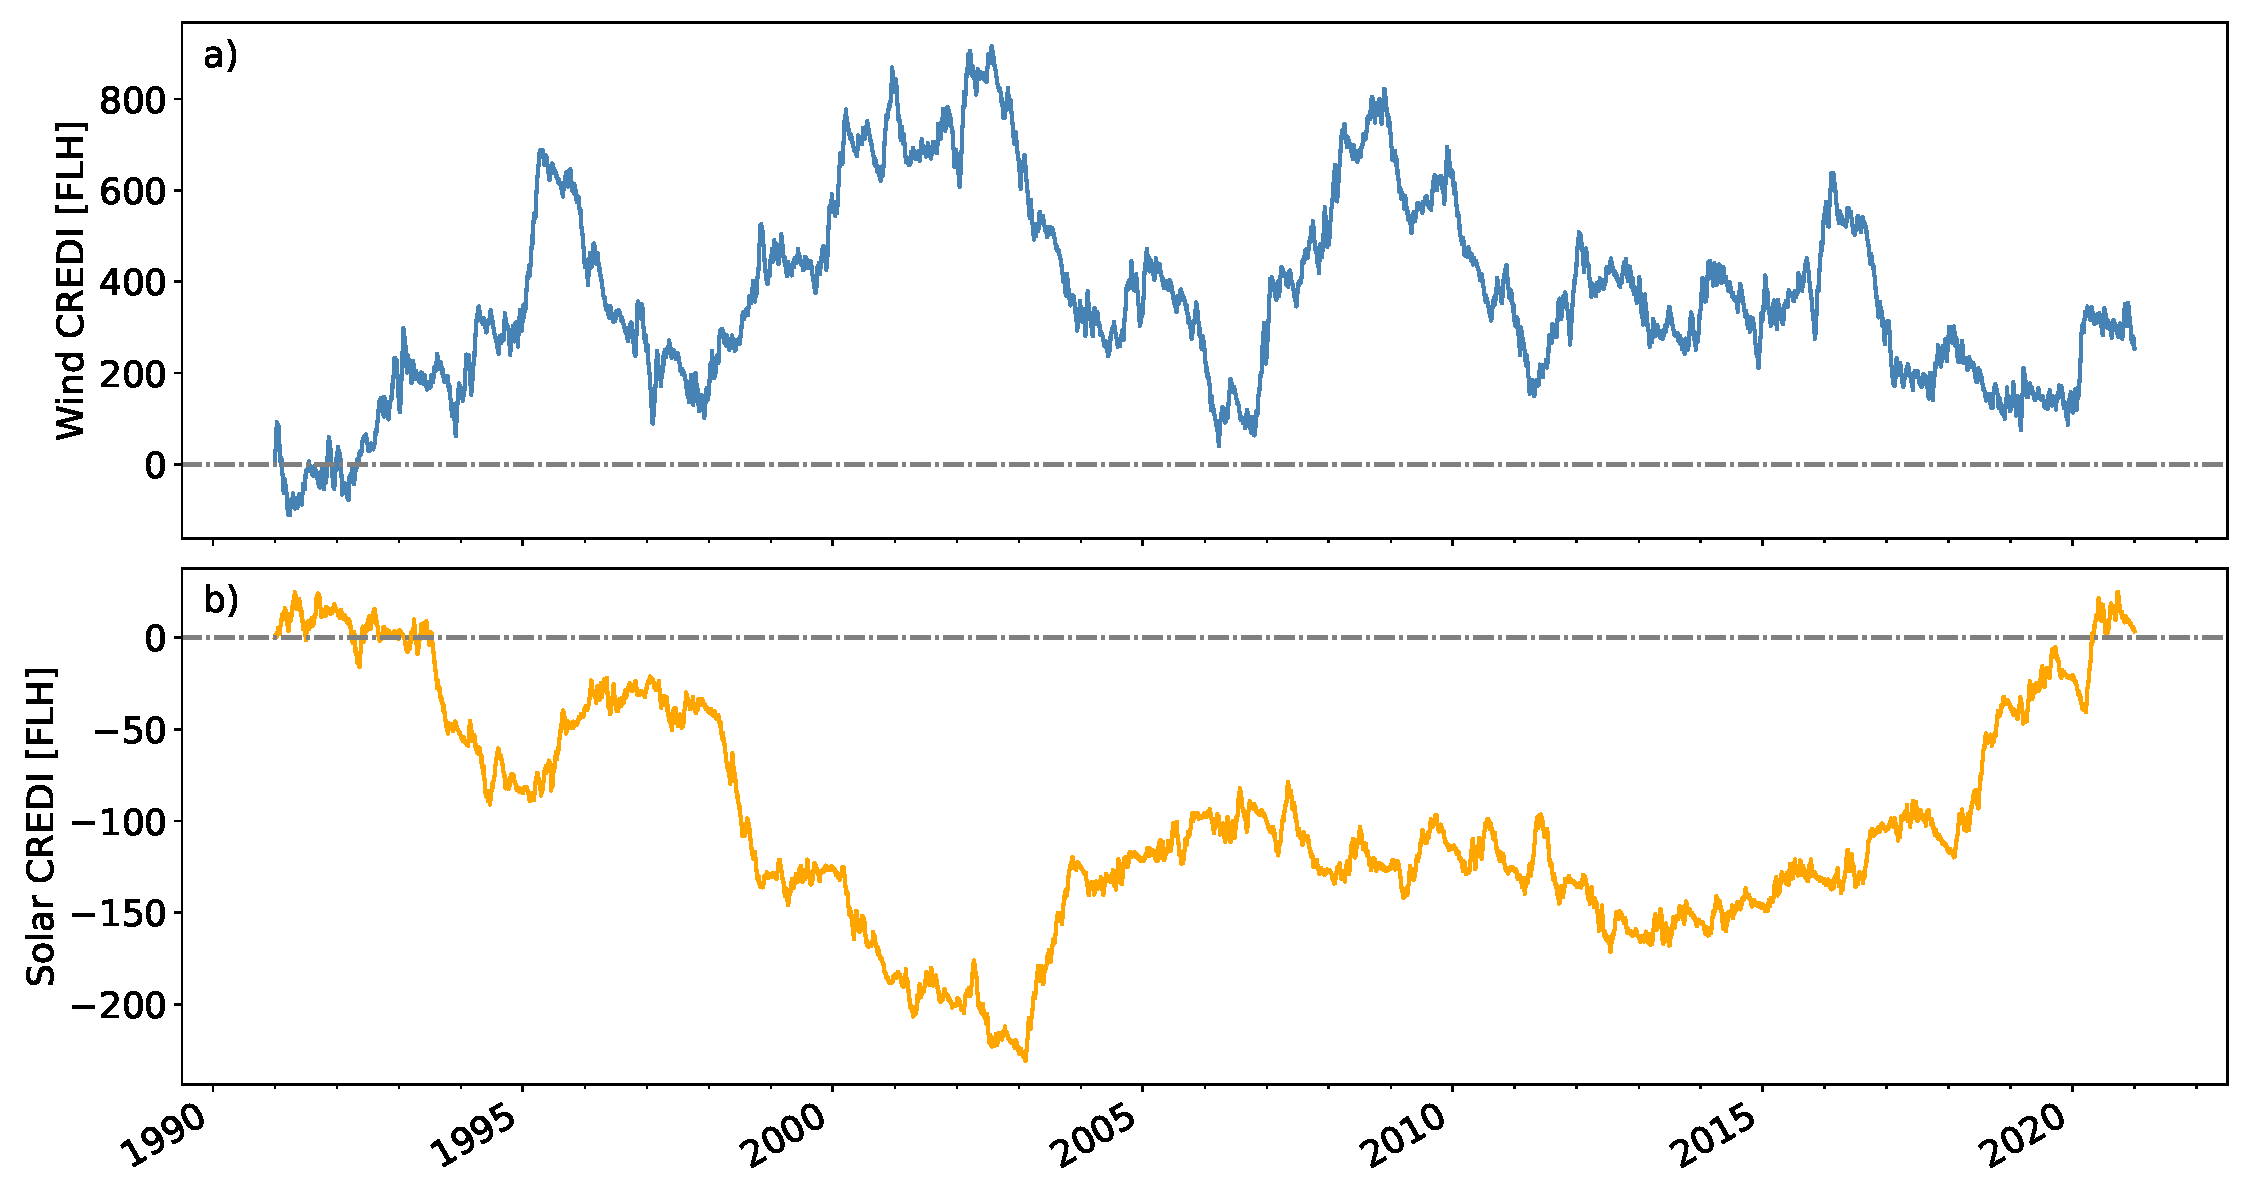
\includegraphics[width=\textwidth]{Figures/CREDI_interannual.pdf}
        % 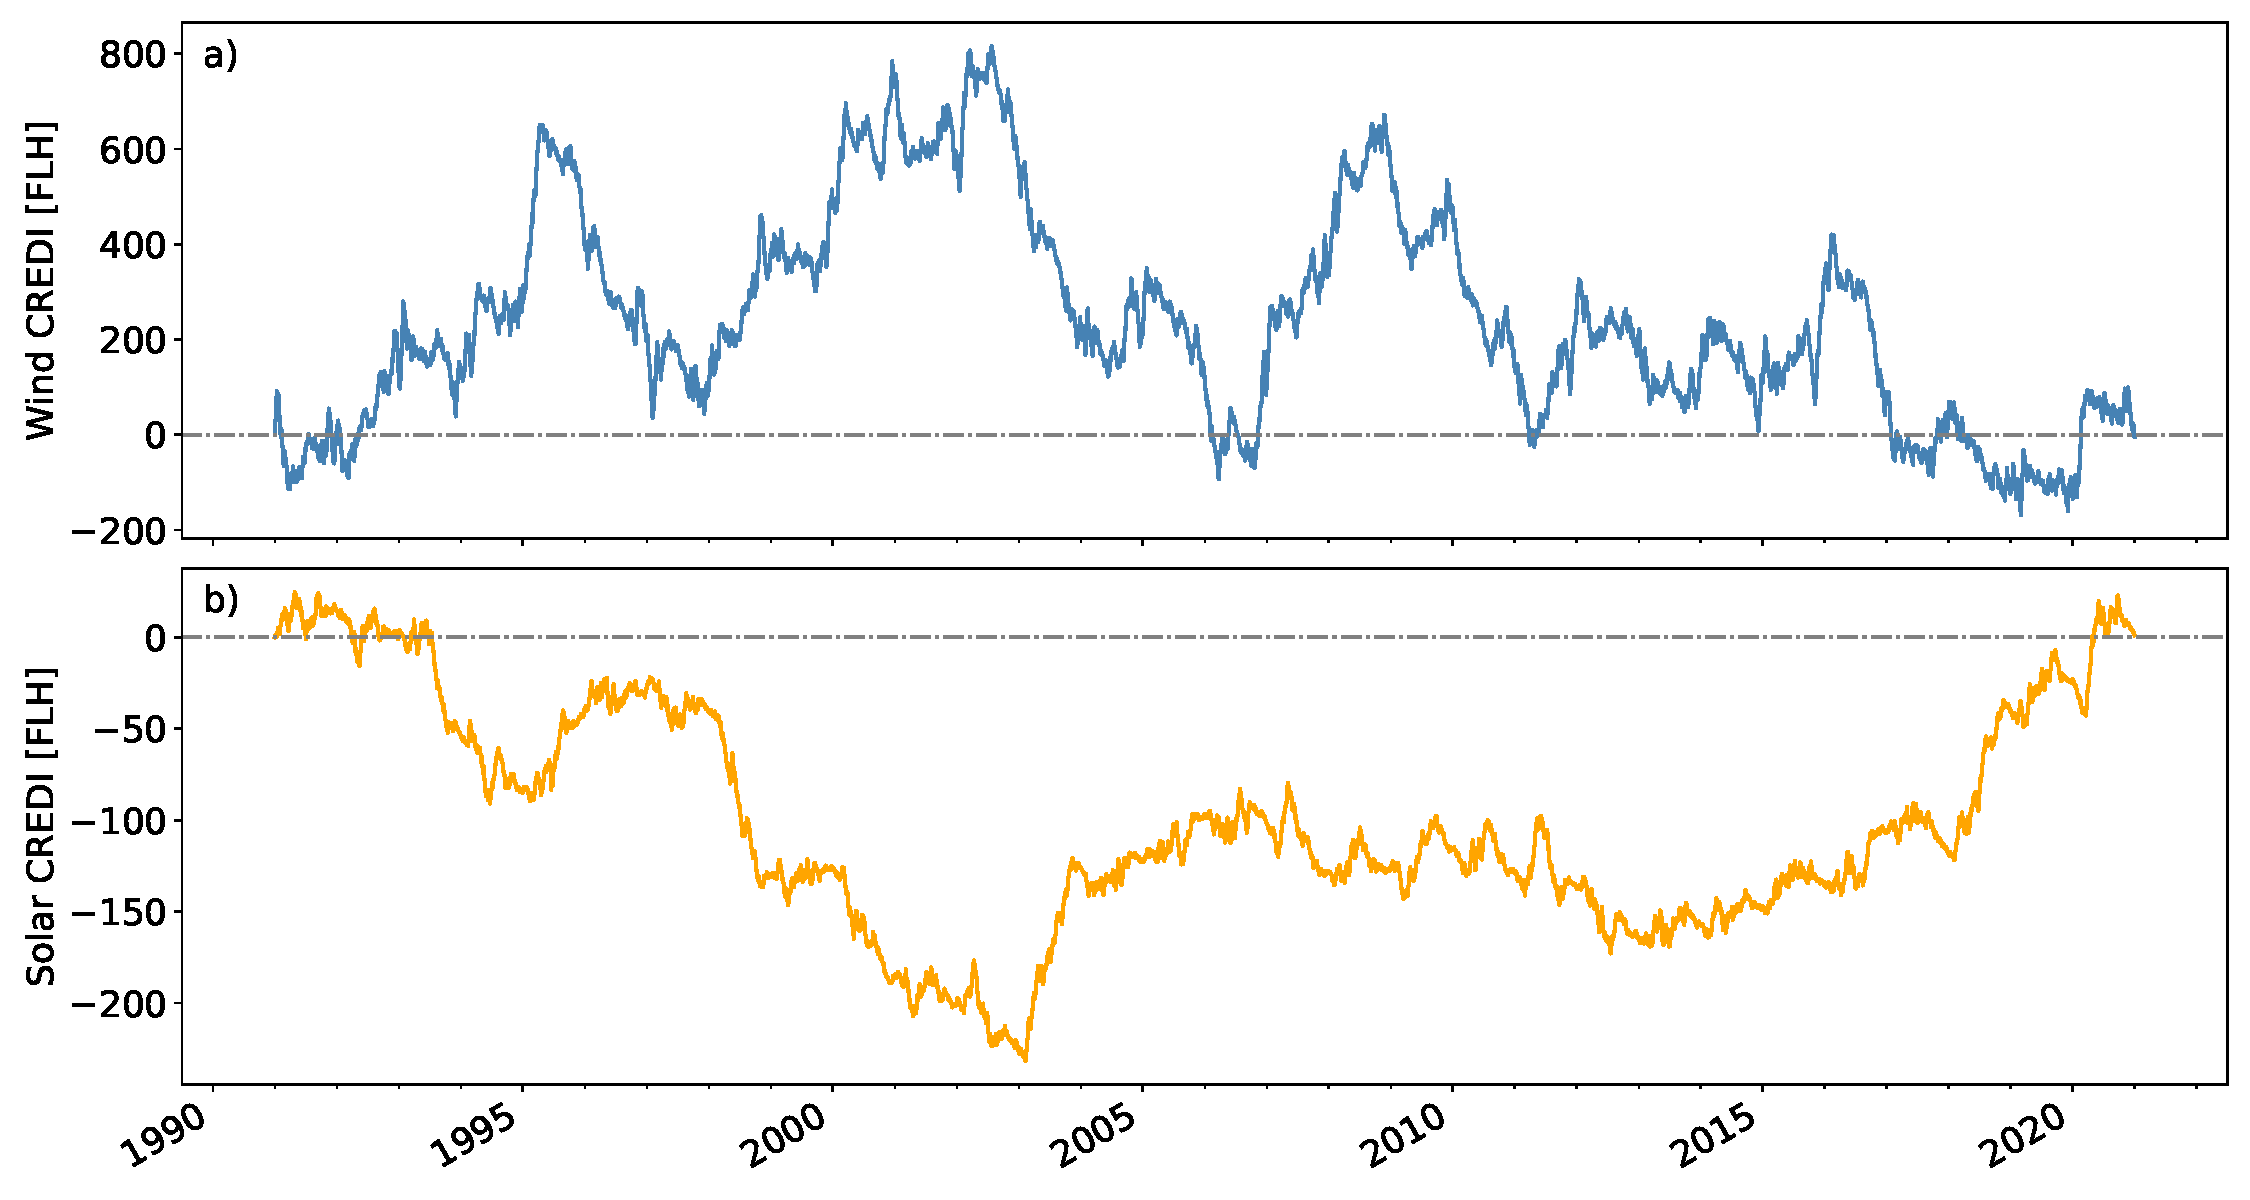
\includegraphics[width=\textwidth]{Mainmatter/CP2/Figures/CREDI_interannual.pdf}
        \caption{
                Hourly Wind (a) and Solar (b) \credi{} over the period 1991-2020 for `NL01'. 
                As the climate was calculated over the same period, by definition the \credi{} sums to zero over the full period.}
        \label{fig:analysis_decadal}
\end{figure}

% A note on unit size, stability & multi-year
The values of \sdi{} are generally lower than those of the \wdi{}. 
This is directly related to the diurnal cycle, which by definition gives zero solar potential at night and low values in the morning and evening. 
Consequently, the sum of the anomalies over a given period is smaller than for wind potential, which has values for all 24~hours in a day.

% General behaviour
Finally, while the impact of the relative observed variability depends on the ratio of installed capacities, we observe that the inter-annual energy-meteorological variability is mainly driven by the wind resource in the analysed region (i.e., the north-west of the Netherlands). 
And though the {\sc wind} and {\sc solar} \credi s show strong anti-correlated behaviour during some years (e.g. from 1991 to 2002), in others this is not the case (e.g. from 2004 to 2005). 
At decadal timescales, wind and solar balance the system somewhat, but they are not suited to fully negate the variability of their counterpart.







%%%%%%%%%%%%%%%%%%%%%%%%%%%%%%%%%%%%%%%%%%%%%%%%%%
%%%%		~~~~ Application: seasonal

\subsection{Seasonal variability in \credi}\label{sc:seasonal}
% INTRO  Consideration when applying CREDI at seasonal scale
When assessing the seasonal energy-meteorological variability using the \credi, the starting point determines the way the temporal development of the index is perceived. 
In line with definitions of hydrological drought, the starting point determines the separation between energy surplus (wet) and deficit (dry) years. 
As the index is intended to capture the energy-meteorological variability, the start date is picked such that the biggest range if \credi{} at the end of, and throughout, the year is observed. 

% Chosen start point
Comparing \credi{} starting points for each month of the year, we found that these should \emph{not} be the same for wind and solar (SI Section B). 
We use May 1\ts{st} as the starting point for wind, as it gives the widest distribution of the index at the end of the analysis window in this particular region.  
For solar no clear distinction is found between a December or January starting point, we chose to use January 1\ts{st} here.

% WIND
For the yearly \wdi, it is obvious that an individual year can either be anomalously positive or negative, and that variations throughout a year are large (Figure~\ref{fig:analysis_seasonal_wind}a). 
This results in a wide range of yearly storylines. 
The 25-75\% spread of the index grows to $\pm180$ FLH over a year (Figure~\ref{fig:analysis_seasonal_wind}b). 
The most extreme negative year in the period considered for \wdi{} was 2016. 
In that year, from about September onwards, the wind potential was almost consistently below expected with $350$ less FLHs at the end of the analysed period.

\begin{figure}[b]
        \centering
        \includegraphics[width=\textwidth]{Figures/WindCREDI_annual}    
        % \includegraphics[width=\textwidth]{Mainmatter/CP2/Figures/WindCREDI_annual}
        \caption{
                Hourly \wdi{} per analysis year over the period May 1991 to April 2021 for `NL01'. 
                Figure a) shows the specific progression of \wdi{} for each year (blue lines). 
                Figure b) shows the distribution of the \wdi{} for each hour of the year, namely the 50\ts{th} percentile (blue line), the 25-75, 10-90 percentile and min-max range (shaded blue, see legend). 
                Four exemplary storylines are shown, namely 1996 (red), 1998 (green), 2003 (purple) and 2016 (black).
        }
        \label{fig:analysis_seasonal_wind}
\end{figure}

% Wind on 1996
As an example of the use of \wdi{} for storyline analysis we look at 1996. From May to October the index is relatively flat, indicating that the wind potential was as expected from its climate (red line in Figure~\ref{fig:analysis_seasonal_wind}b). 
Then, a strong reduction is observed in the \wdi{} from December to the end of January, indicating much lower then average potential generation from wind. Part of this deviation is compensated by higher than normal generation potential in February of 1997.

% SOLAR + interp
As noted earlier, values of yearly \sdi{} are smaller than of \wdi{} (Figure~\ref{fig:analysis_seasonal_solar}a), with an average spread (25-75\%) of $\pm18$~FLHs, and uncommon spread (10-90\%) of $\pm35$~FLHs spread over a year (Figure~\ref{fig:analysis_seasonal_solar}b). 
This indicates that \textasciitilde18~FLHs of total energy is needed to cover the deficit of the installed solar capacity in 50~\% of years and \textasciitilde35~FLHs to cover 80\% of years (Figure~\ref{fig:analysis_seasonal_solar}). 

% solar extreme
The most extreme year of high solar potential was 2003; the most extreme year of low solar potential was 1998. 
Especially 2003 is remembered for its extremely warm and sunny summer \parencite{GarcaHerrera2010}.

\begin{figure}[t]
        \centering
        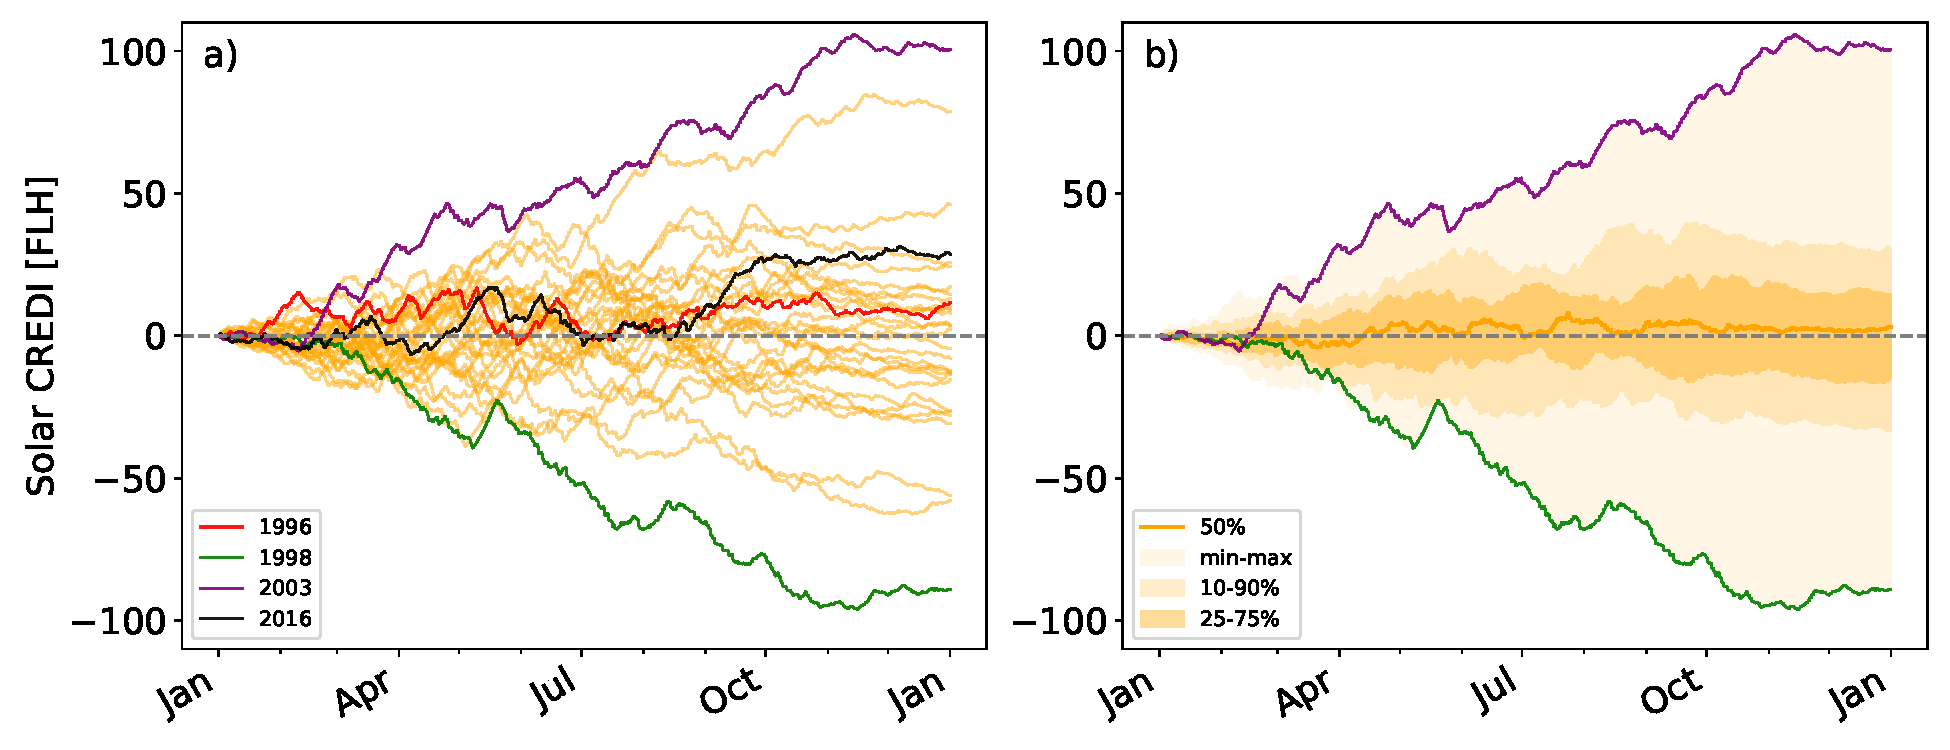
\includegraphics[width=\textwidth]{Figures/SolarCREDI_annual} 
        % 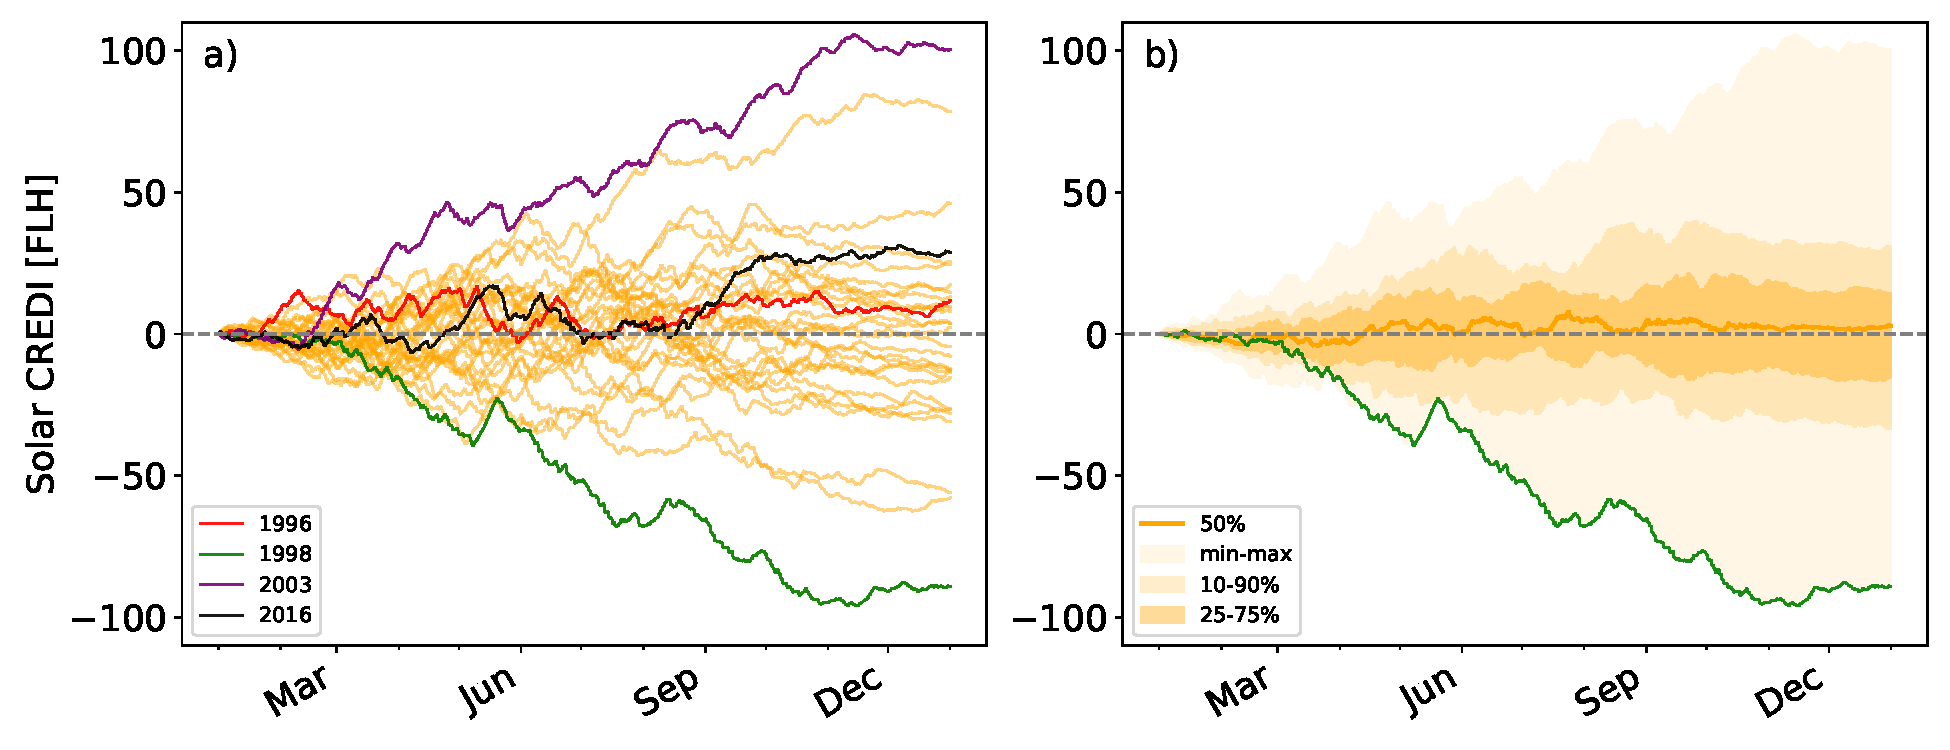
\includegraphics[width=\textwidth]{Mainmatter/CP2/Figures/SolarCREDI_annual}
        \caption{
                Hourly \sdi{} per year over the period 1991-2020 for `NL01'. 
                As shown in Figure~\ref{fig:analysis_seasonal_wind}, but the \sdi{} is shown in orange hues.
        }
        \label{fig:analysis_seasonal_solar}
\end{figure}







%%%%%%%%%%%%%%%%%%%%%%%%%%%%%%%%%%%%%%%%%%%%%%%%%%
%%%%		~~~~ Application: Sub-seasonal
\subsection{Sub-seasonal variability in \credi}\label{sc:subseasonal}

% INTRO Consideration when applying CREDI at sub-seasonal scale
At sub-seasonal timescales, similar to seasonal, the start point determines the way the temporal development of the index is perceived. 
We use 'energy'-seasons to capture the large scale changes on sub-seasonal timescales. 
For wind we define two seasons of interest: September to March, and April to August. 
For brevity, only the results found for wind in the winter `energy'-season are shown here, see SI Section C for the other and solar. 
Alternative definitions of 'energy'-seasons can be relevant, especially for regions that have different sub-seasonal behaviour then the `NL01'-region shown here.

% WIND For WEB at sub-seasonal scale
It is obvious that different years show quite different characteristics (Figure~\ref{fig:analysis_sub-season-winter_wind}a) and individual winter seasons can differ greatly. 
As expected, the sub-seasonal timescale is emphasised more. 
For instance, the anomalous index-development in 1996 described in Section~\ref{sc:seasonal} is more clearly visible. 
Especially the strong reduction in \wdi{} from December to the end of January stands out as a period of much lower than normal wind generation potential.

\begin{figure}[t]
        \centering
        \includegraphics[width=\textwidth]{Figures/WindCREDI_seasonal-winter} 
        % \includegraphics[width=\textwidth]{Mainmatter/CP2/Figures/WindCREDI_seasonal-winter}
        \caption{
                Hourly winter \wdi{} per season (Sep.-Apr.) for 1991-2021 for `NL01'. 
                Figure a) shows the specific progression of \wdi{} for each summer season (blue lines). 
                In addition, four example storylines are represented, namely those starting in 1996 (red), 1998 (green), 2003 (purple) and 2016 (black). 
                Figure b) shows two storylines (1996, 2003) and the hourly distribution of the \wdi{}, namely the 50\ts{th} percentile (blue line), the 25-75, 10-90 percentile, and min-max range (shaded blue, see legend).
        }
        \label{fig:analysis_sub-season-winter_wind}
\end{figure}


%%%%%%%%%%%%%%%%%%%%%%%%%%%%%%%%%%%%%%%%%%%%%%%%%%
%%%%		~~~~ Application: Short-term / events

\subsection{A short-term study window for event-based \credi{}}\label{sc:shortterm}
% short-term
Finally, short-term events, e.g. \emph{Dunkelflautes}, can pose significant risk to highly renewable energy systems \parencite{tedesco2023,Mockert2022arxiv,vanderwiel2019extreme,Li2022,Sundar2022}. 
A 8-day window for \credi{} aligns with previous work~\parencite{tennet2023}, and is investigated here, see SI Section D for additional figures and the top 50 8-day events. 

% Showcase not all storylines, many overlap -> filter
For short-term event analysis we do not pre-define the start point, all 8-day windows are considered. 
Overlapping events that share a five or more days, are removed from the analysis. 
While we only consider the lowest final \credi{} value for our event selection, other impact selection methods as described by \textcite{vanderWiel2021} can be used.

% Observations general
Again we noted the large weather-caused variability between different 8-day periods (Figure~\ref{fig:analysis_short-term-winter_wind}a). 
The computed spread in Figure~\ref{fig:analysis_short-term-winter_wind}b considers events throughout the year. 
This can also be investigated on a seasonal basis for winter or summer-specific event information, or for shorter or longer events.  

% Observations specific
The most extreme event is from 16-24 jan. 2017 and the analysis year 2016 is present 3 times in the top 50 events. 
While the specific 8-day event found in \textcite{tennet2023} is not the most extreme event, the analysis year 1996 does show up four times in the top 50 events. 
Indicating that the analysis year 1996 indeed stands out as quite exceptional.

%% short-term
\begin{figure}[t]
        \centering
        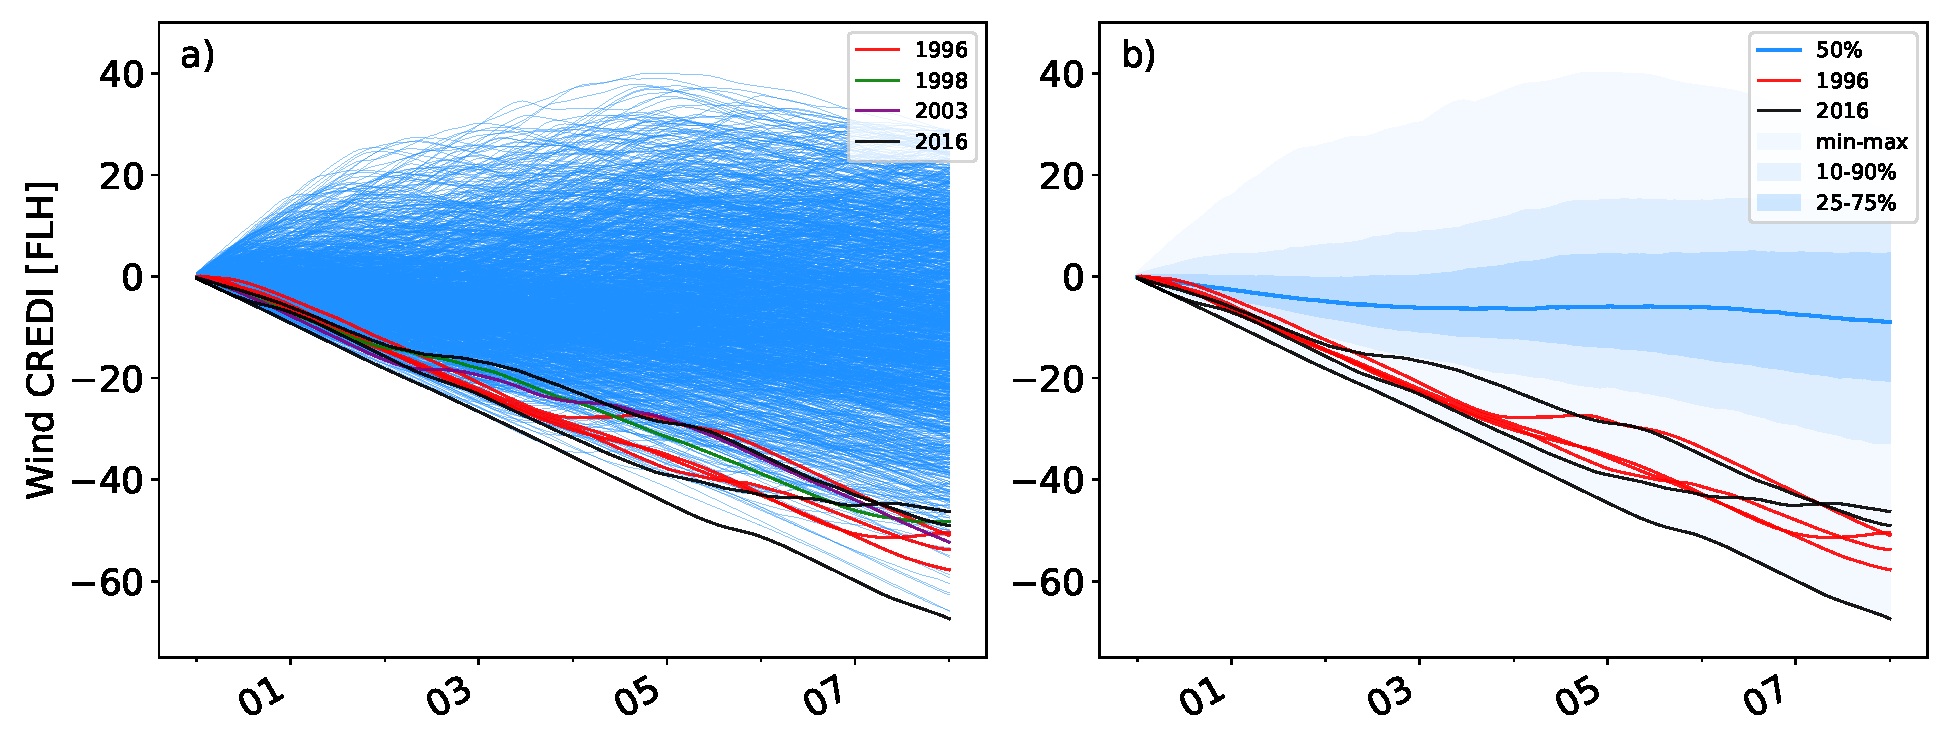
\includegraphics[width=\textwidth]{Figures/WindCREDI_shortterm}
        % 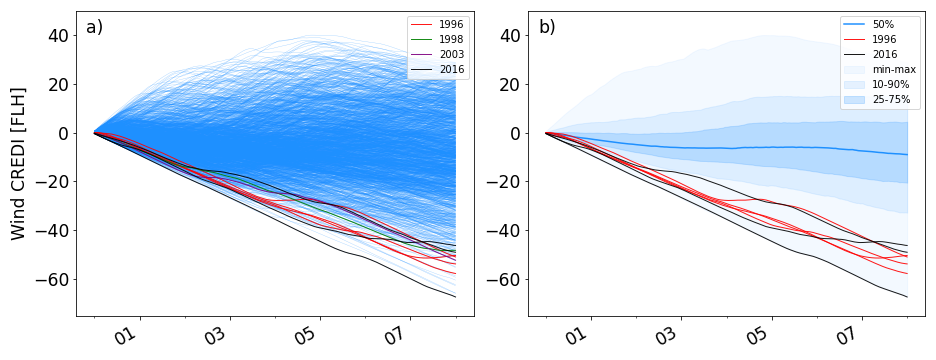
\includegraphics[width=\textwidth]{Mainmatter/CP2/Figures/WindCREDI_shortterm}
        \caption{
                Hourly winter \wdi{} during 8-days for all events with less then 5 days overlapping in the period May 1991 to April 2021 for `NL01'. 
                The storylines show the analysis years 1996 (red, 4x), 1998 (green, 1x), 2003 (purple, 1x) and 2016 (black, 3x). 
                Furhter formatting as shown in Figure~\ref{fig:analysis_sub-season-winter_wind}.
        }
        \label{fig:analysis_short-term-winter_wind}
\end{figure}








%%%%%%%%%%%%%%%%%%%%%%%%%%%%%%%%%%%%%%%%%%%%%%%%%%
%%%%		~~~~ Discusssion ~~~~
%%%%%%%%%%%%%%%%%%%%%%%%%%%%%%%%%%%%%%%%%%%%%%%%%%

\section{Discussion}\label{secCP2:discussion}
% Depends on climate definition, options to improve this
The presented index is defined as the cumulative anomaly of a renewable resource with respect to its climate. 
The method of determining the climate is thus vital and, as shown, should take into account the strong diurnal and annual cycle present in renewable energy resources. 
The calculation of the climate used here has a dependence on the size of the rolling window, which was primarily based on expert judgement. 
A longer timeseries, covering many decades, could be used for a cross-validation check to obtain the optimum \emph{rolling window} size, but the data source should be selected with great care, due to potential inconsistencies~\parencite{wohland2019significant,Wohland2022,Deser2023}. 
In previous work a climatic definition on harmonics has been effective~\parencite{Sabziparvar2014,Fischer2019,Rayson2021}, but we found it unsuitable here (see SI Section A.B). 

% Index only shown on hour, shorter needs more work
When combined with weather forecasts, indices for hydrological drought can help policy makers make early decisions regarding societal risks~\parencite{Quiring2009,Stagge2015,Cammalleri2021,vanderWiel2022}. 
However, the operation of the electricity grid requires balance on very short timescales~\parencite{craig2022disconnect,tennet2023}. 
While we presented our index with an hourly resolution, further research is needed to investigate if the \credi{} can also be applied on these very short timescales. 
The examples provided, however, do already show \credi's usefulness in resilience planning, resource adequacy assessments, and as a metric for selecting events for robustness analysis.

% Meteo & Energy differs per region, so region specific approach needed
In this introduction of the index, we applied it to the north-west region of the Netherlands. 
However, as shown by \textcite{Pickering2020}, energy-meteorological variability is strongly region dependent. 
Therefore, the \credi{} should be calculated and analysed for each region separately. 
Due to the ease of application, and the intuitive analysis and interpretation of the index, this application to other regions is relatively straightforward (see SI Section E for a few additional regions). 




%%%%%%%%%%%%%%%%%%%%%%%%%%%%%%%%%%%%%%%%%%%%%%%%%%
%%%%		~~~~ Conclusion ~~~~
%%%%%%%%%%%%%%%%%%%%%%%%%%%%%%%%%%%%%%%%%%%%%%%%%%


\section{Conclusion}\label{secCP2:conclusion}
% General conclusion
Drawing inspiration from the work on drought monitoring indices, we have presented the Climatological Renewable Energy Deviation Index (\credi{}). 
This new index is meant as an analytical method for researchers and stakeholders to help them understand and explain the impact of the variable nature of the weather on the energy system. 
The index computes the cumulative deviation or anomaly from the mean expected weather (its climate) for a chosen period. 
Given the relevance of both the diurnal and annual cycle in meteorology for energy applications, we recommend a simple but suitable definition of the background climate using an hourly rolling window approach. 

% Other applications
The index can be used when understanding of energy-meteorological variability is key. 
For example, the \credi{} can be used as part of a resource adequacy analysis from TSOs to identify events which are likely to be a challenge in maintaining security of supply in a (future) power system driven by renewable energy sources. 
At the same time, the \credi{} could be used to assess the volume and power output of back-up resources needed for a given timescale, region, and energy system design.
Then, by using the event selection and analysis, as e.g. in \textcite{vanderWiel2021} for hydrological extremes, detailed event descriptions can be developed, systems can be stress tested, and further insight could be gained into energy-meteorological variability.





%%%%%%%%%%%%%%%%%%%%%%%%%%%%%%%%%%%%%%%%%%%%%%%%%%
%%%%		~~~~ Backmatter ~~~~
%%%%%%%%%%%%%%%%%%%%%%%%%%%%%%%%%%%%%%%%%%%%%%%%%%

% Contribution statement
\section*{CRediT Author Statement}
Conceptualisation, Formal Analysis and Visualisation: LPS, Investigation, Methodology and Writing - Original Draft: LPS, KvdW, Writing - Review \& Editing: \emph{All listed authors}, Supervision and Funding acquisition: \emph{AJF, MvdB}. 

% Acknowledgement section
\ack 
Laurens P. Stoop received funding from the  Dutch Research Council (NWO) under grant number 647.003.005. 
The content of this paper and the views expressed in it are solely the author’s responsibility, and do not necessarily reflect the views of TenneT TSO B.V..

% Statement on open & FAIR research
\section*{Open research} 
The implementation of the \credi{}, its use at different timescales, all code used to generate the figures, the data from the `NL01' region discussed and the full list of the most extreme short-term events found as presented in this study are available at Github via \url{https://github.com/laurensstoop/ccmetrics} with the MIT license. 

The preliminary data of the PECDv4 containing the regional renewable resource potential for historical technological definitions of wind and solar used for in this study to showcase the \credi{} are not available due to ongoing validation. 
In due time the full PECDv4, including raw gridded and aggregated regional/national renewable resource potentials for a wide range of technological definitions, will be made available as part of the C3S Energy dataset and can be found through \url{https://climate.copernicus.eu/operational-service-energy-sector}. 


% Now as an seperate file for SI
\appendix
\section{Supporting Information}
Supporting Information related to this article can be found online. %  at \url{https://doi.org/10.nnnn/ppppp}.


% common bib file
\printbibliography 




\end{document}





